\documentclass[10pt]{beamer}
\usetheme{Malmoe}
\colorlet{beamer@blendedblue}{green!40!black}
\setbeamertemplate{navigation symbols}{}
\newcommand*\oldmacro{}%
\let\oldmacro\insertshorttitle%
\renewcommand*\insertshorttitle{%
\oldmacro\hfill%
\insertframenumber\,/\,\inserttotalframenumber}

\usepackage{caption}
\usepackage{hyperref}
\usepackage[makeroom]{cancel}
\usepackage{ amssymb }
\usepackage{appendixnumberbeamer}
%\usepackage{tikz-feynman}
\usepackage{graphicx}
\begin{document}
\title{Search for Flavor Changing Neutral Currents in Top Quark Decays}
\subtitle{$t \rightarrow q \gamma$}
\author[Barkeloo]{Jason Barkeloo}

\titlegraphic{
\includegraphics[width=4cm]{../ATLAS-Logo-Ref-RGB.png}\hspace*{2.75cm}~%
   
\includegraphics[width=4cm]{../uo_logo_green_on_white_2.jpg}
}

%\frame{\frametitle{}
%\begin{itemize}
%\item
%\end{itemize}
%}


\date{November 15, 2018}
\frame{\titlepage}
\frame{\frametitle{Overview}\tableofcontents[]}%hidesubsections]}
\section{Brief Background}
%\frame{\frametitle{Table of Contents}\tableofcontents[currentsection,hideothersubsections]}
%%%%%%%%%%%%%%%%%%%%%%%%%%%%%%%%%%%%%%%%%%%%%%%%%%%%%%%%%

\subsection{The Top Quark}

\frame{\frametitle{Top Quark Pair Production}
\begin{itemize}
\item Leading order processes for top quark production
	\begin{itemize}
	\item Quark-antiquark annihilation $\approx 10\%$
	\item Gluon-gluon fusion $\approx 90\%$
	\end{itemize}
\end{itemize}
\centering

	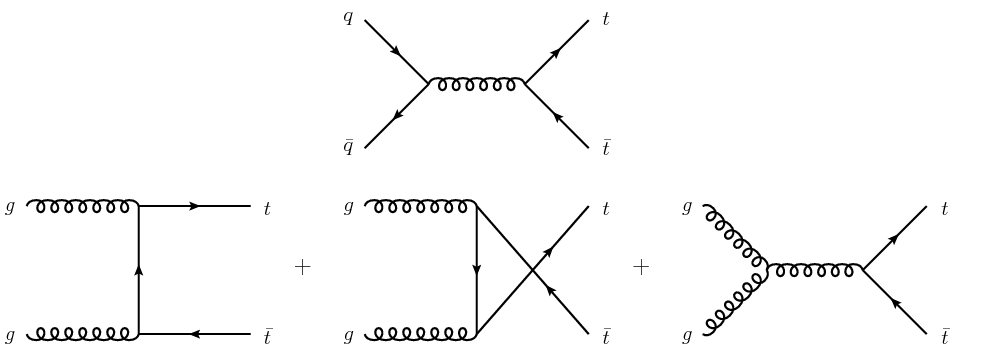
\includegraphics[height=0.5\textheight]{../../Thesis/ThesisImages/LOPairProdDiags.png}
	\captionof{figure}{Leading order $t\bar{t}$ diagrams}
}

\frame{\frametitle{Top Quark Pair Production}
\begin{itemize}
\item At $\sqrt{s}=13TeV$ for $m_{t}=172.5GeV$, $\sigma_{t\bar{t}} = 831.76pb$
\end{itemize}
\centering
	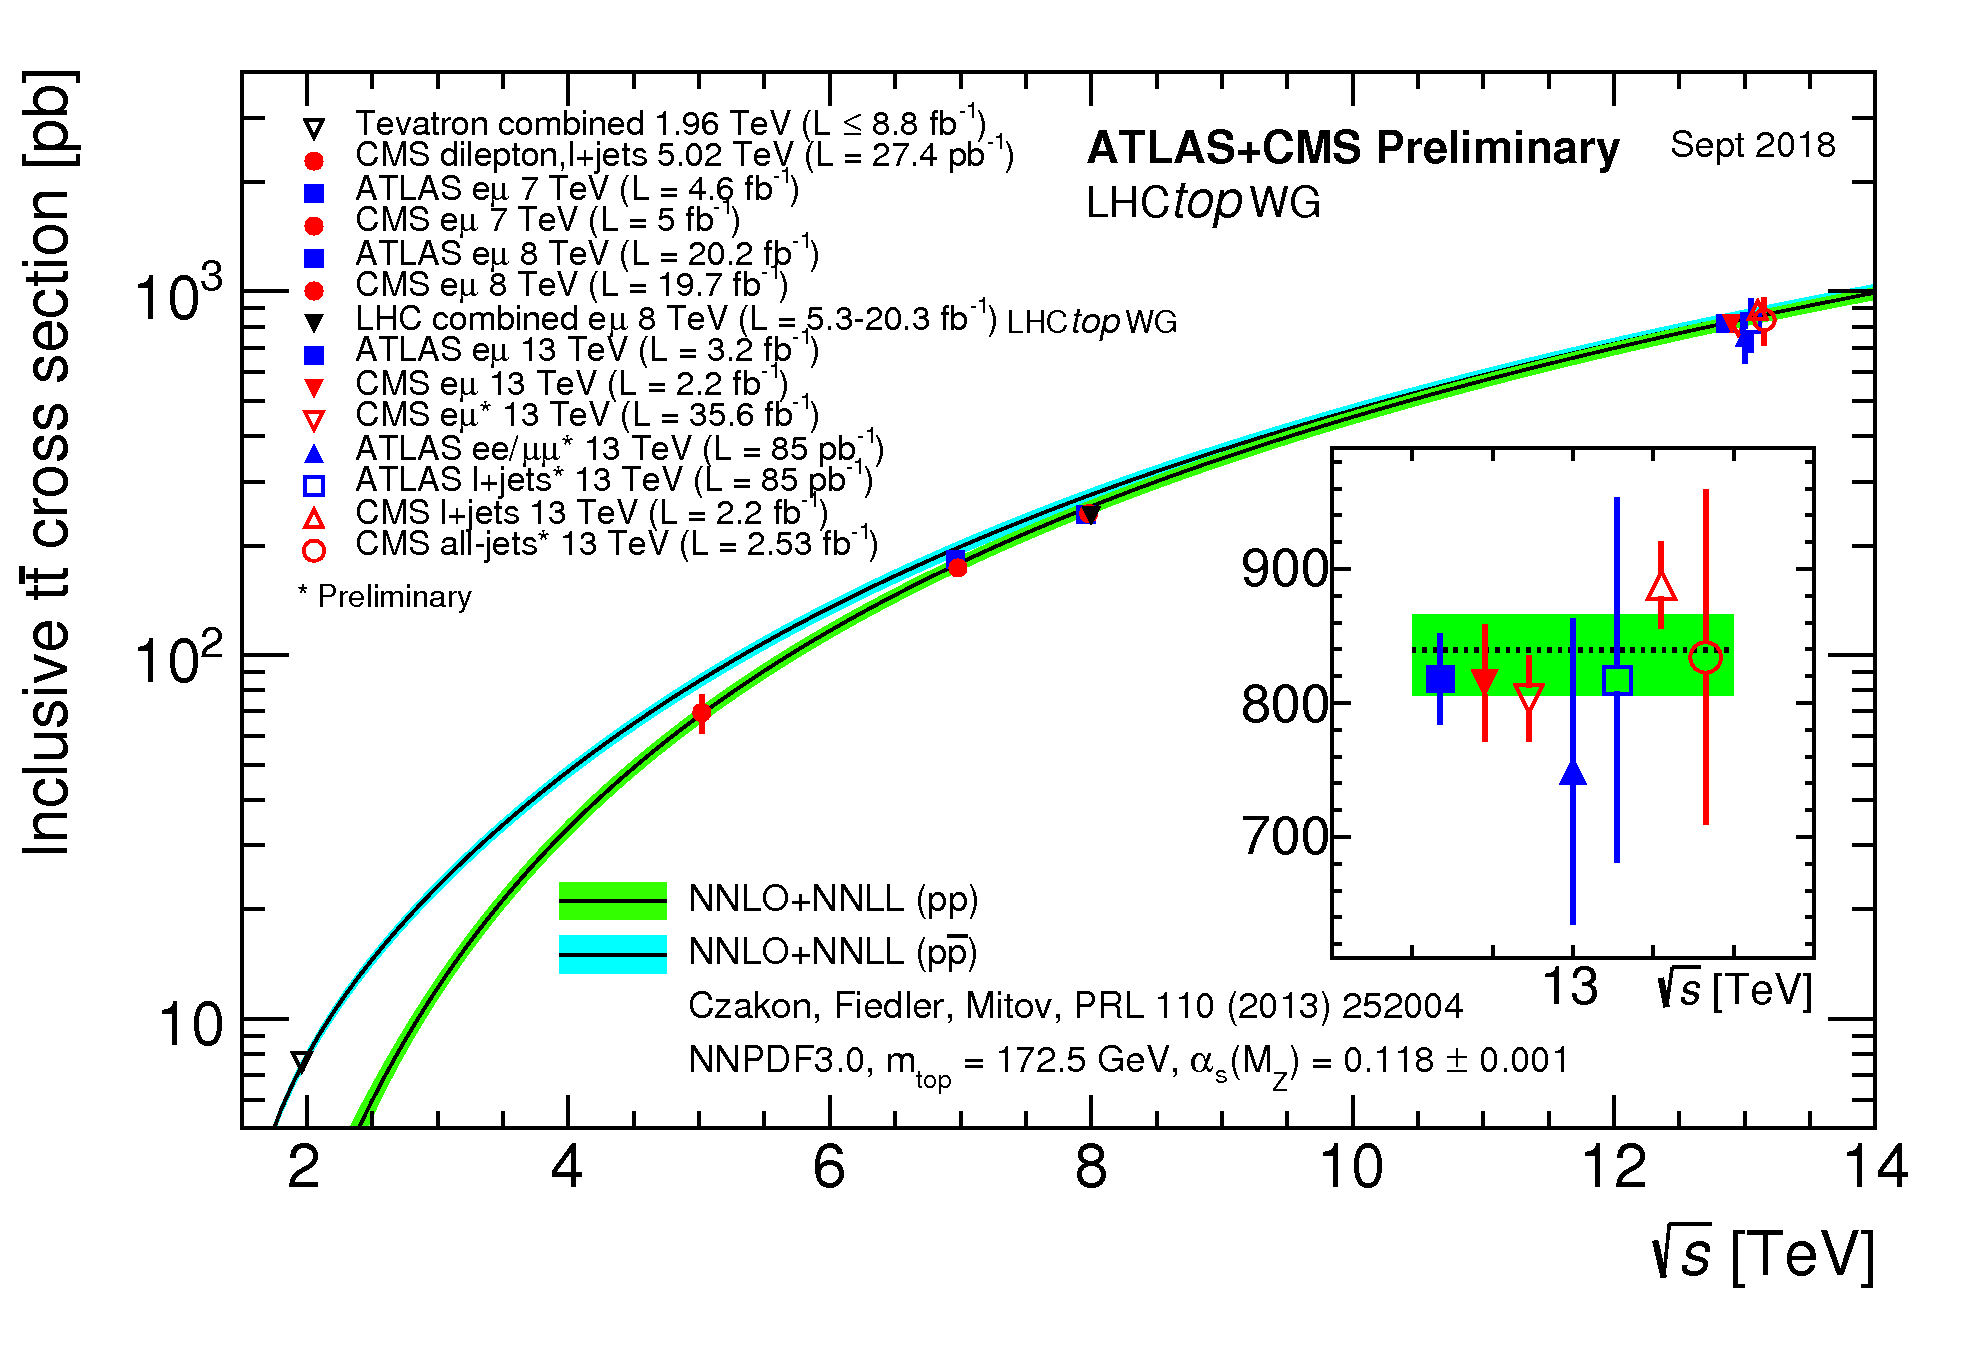
\includegraphics[height=0.7\textheight]{../../Thesis/ThesisImages/ttprodxsec.png}
	\captionof{figure}{$t\bar{t}$ production cross section \href{https://twiki.cern.ch/twiki/bin/view/LHCPhysics/LHCTopWGSummaryPlots}{[TopWGSummaryPlots]}}
}

\frame{\frametitle{Top Quark Decays}
\begin{columns}
\begin{column}{0.5\textwidth}
\begin{itemize}
\item Standard model top branching ratio to bW $\simeq 100\%$
\end{itemize}
\centering
 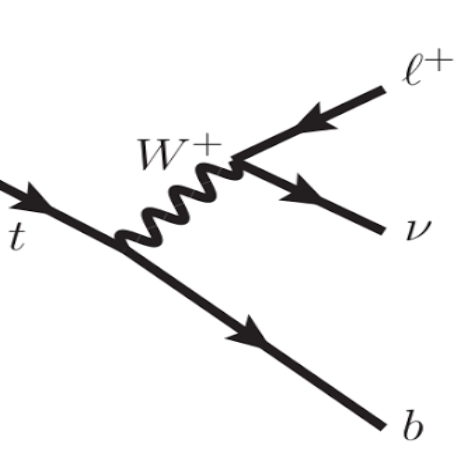
\includegraphics[width=0.7\textwidth]{../../Thesis/ThesisImages/topdecay.png}
 \captionof{figure}{Leptonic final state diagram for a top decay}
\end{column}
\begin{column}{0.5\textwidth}  %%<--- here
     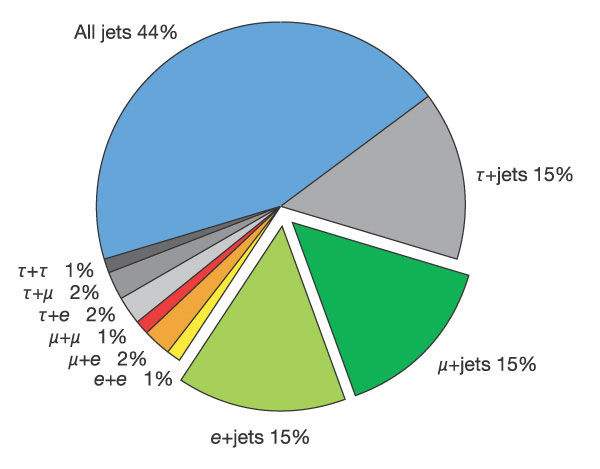
\includegraphics[width=1.1\textwidth]{../../Thesis/ThesisImages/topdecayproducts.jpg}
    \captionof{figure}{Top quark pair decay final states \href{https://images.nature.com/full/nature-assets/nature/journal/v429/n6992/images/nature02589-f2.2.jpg}{[Nature]}}
\end{column}
\end{columns}
}

\frame{\frametitle{Top Quark Decays in the SM}
\centering
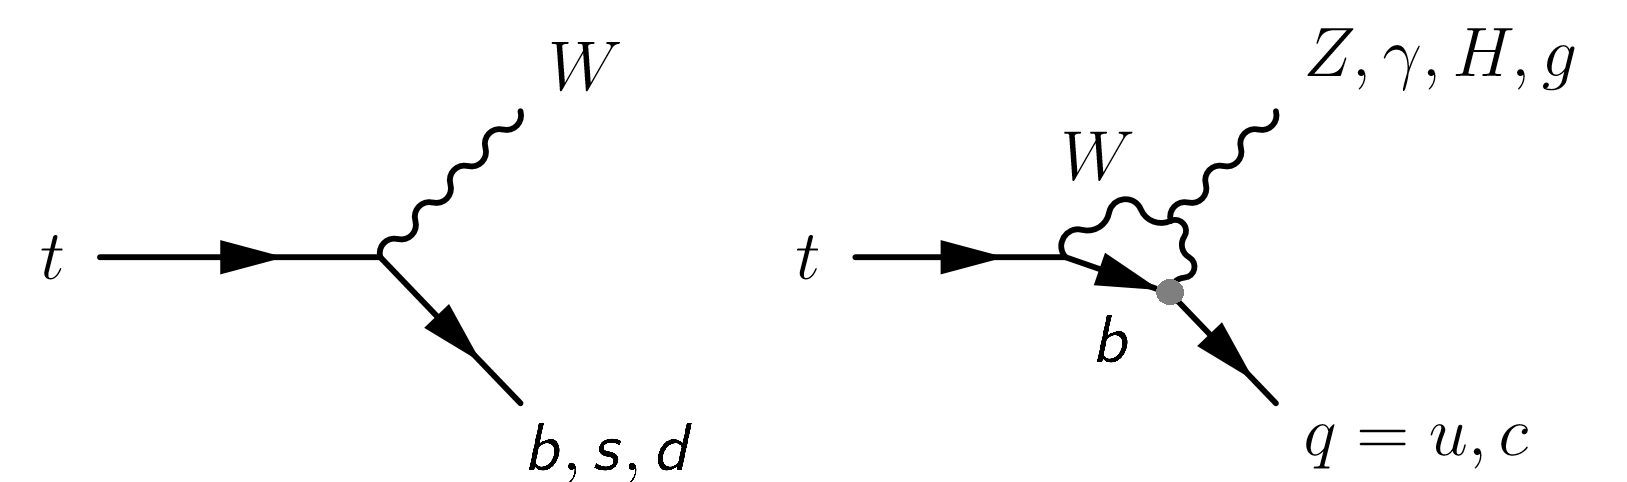
\includegraphics[width=1.\textwidth]{../../Thesis/ThesisImages/SMTopDecays.png}

\begin{columns}
\begin{column}{0.5\textwidth}
\begin{itemize}
\item $t\rightarrow b W \approx 99.83\%$
\item $t\rightarrow s W \approx 0.16\%$
\item $t\rightarrow d W \approx 0.01\%$
\end{itemize}
\end{column}
\begin{column}{0.5\textwidth}
\begin{itemize}
\item $t\rightarrow q_{u,c} X\approx 10^{-17} - 10^{-12}$
\end{itemize}
\end{column}
\end{columns}

%\feynmandiagram [small,horizontal=a to b] {
%  a [particle=\(t\)] -- [fermion] b ,
% f1 [particle=\({b,s,d} \)] -- b -- [boson] f2 [ particle=\(W\)],
%};
}


\frame{\frametitle{Top Flavor Changing Neutral Currents}
\begin{itemize}
\item Current Limits on FCNC Decays
\end{itemize}
\centering
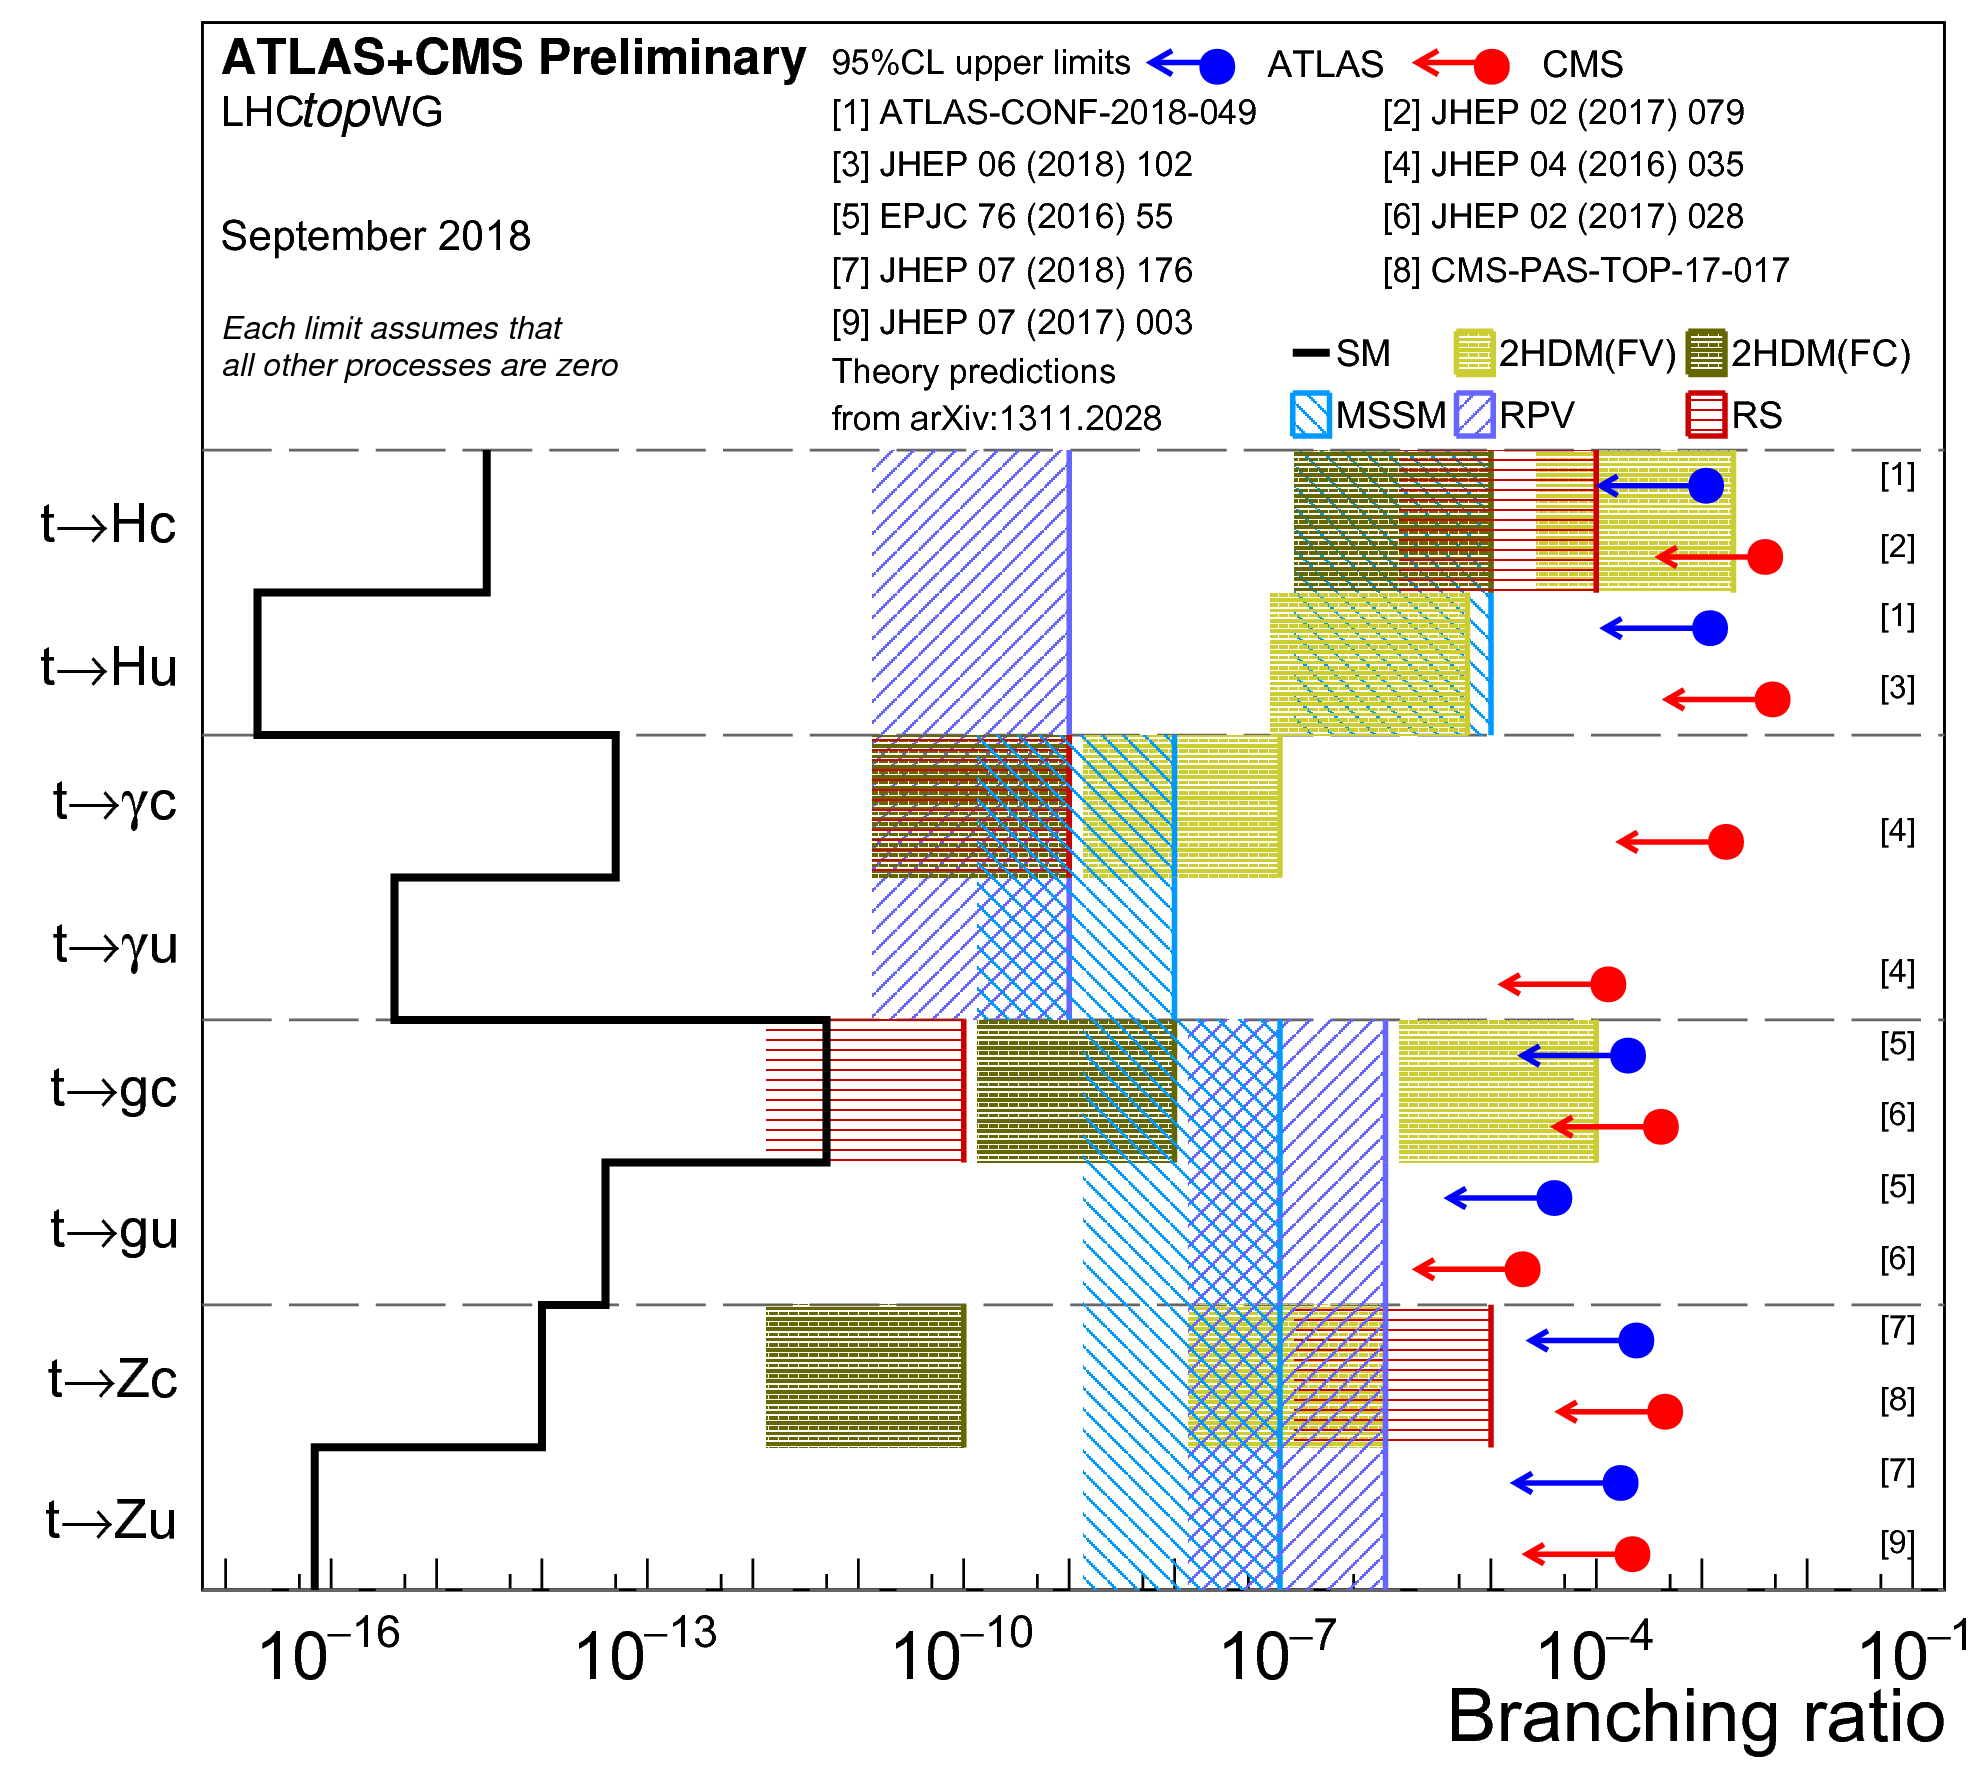
\includegraphics[width=0.55\textwidth]{../../Thesis/ThesisImages/AllFCNCLimits.png}
\begin{itemize}
\item Limits on $t\rightarrow \gamma q$ processes: \href{https://arxiv.org/abs/1511.03951}{[JHEP 04 (2016) 035]}
	\begin{itemize}
	\item $t\rightarrow \gamma u < 1.3 x10^{-4}$
	\item $t\rightarrow \gamma c < 1.7 x 10^{-3}$
	\end{itemize}
\end{itemize}
}


\subsection{FCNC at the LHC}
\frame{\frametitle{FCNC: What are we looking for? $t\bar{t}\rightarrow W (\rightarrow l \nu) b+ q\gamma$}
\begin{itemize}
\item Final state topology
	\begin{itemize}
	\item One Neutrino, from W
	\item One Lepton, from W
	\item One B-jet, SM top
	\item One Photon, FCNC Top
	\item One Jet, FCNC Top
	\end{itemize}
\end{itemize}
\centering
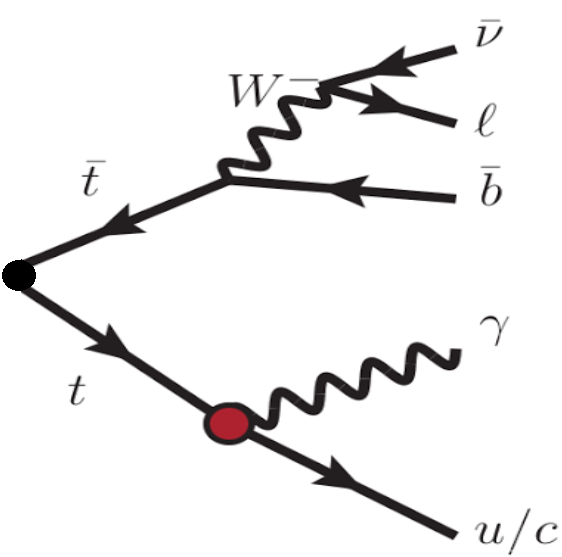
\includegraphics[width=0.4\textwidth]{../../Thesis/ThesisImages/fcncttbar.png}
}

\frame{\frametitle{Background Processes}
\begin{itemize}
\item Due to all of the processes at hadron colliders it is important to model similar event topologies well.
\item Major backgrounds include $t\bar{t}$, W+Jets, Z+Jets, + processes with an associated photon
\end{itemize}
\centering
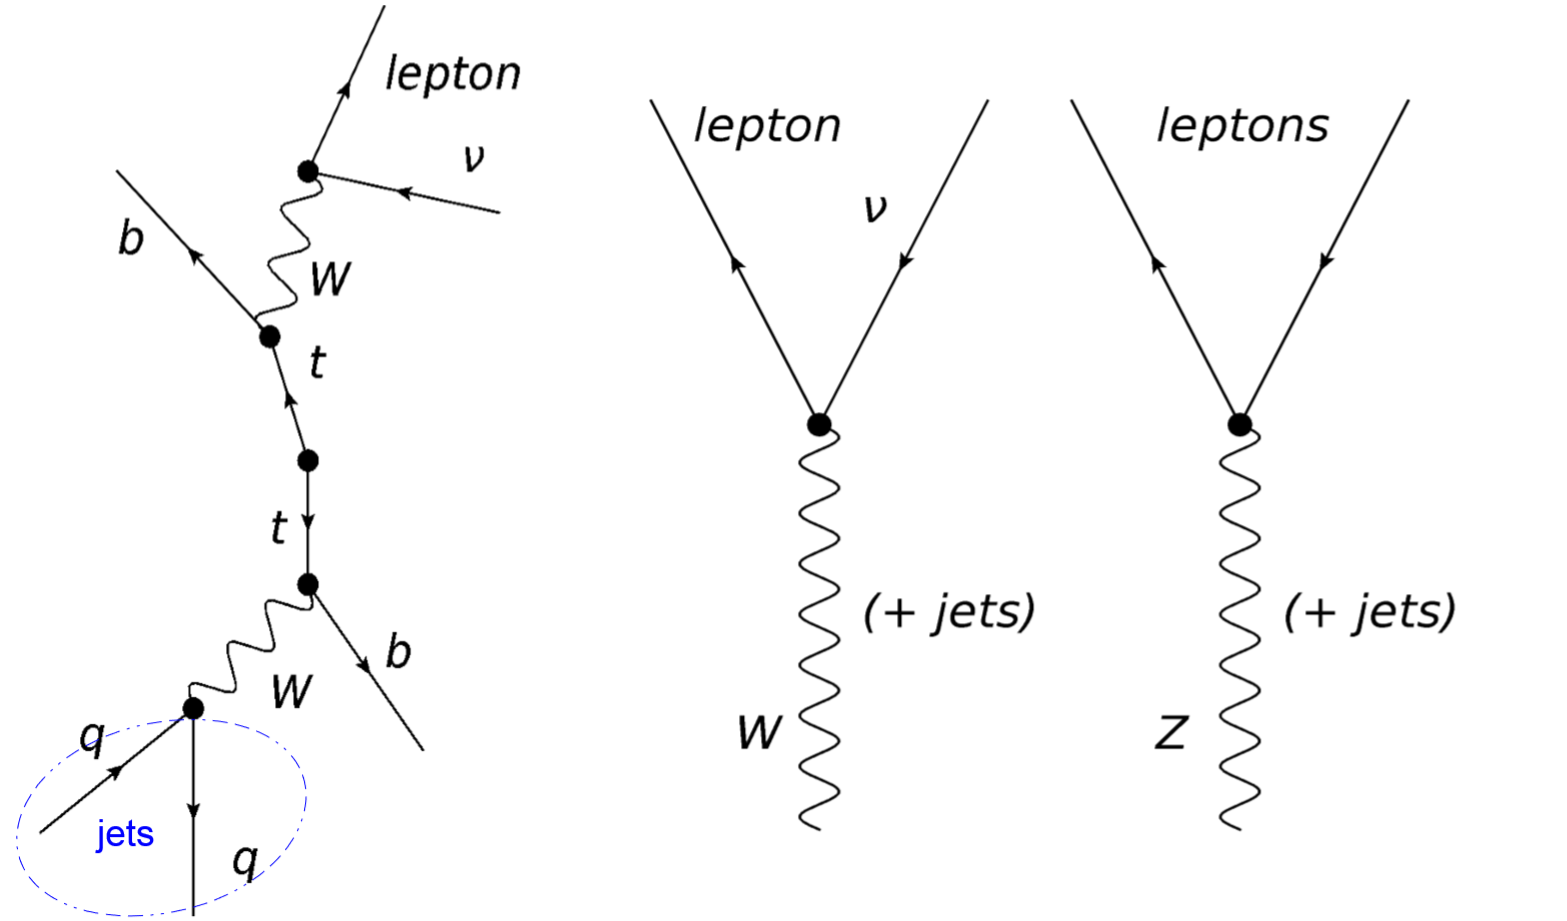
\includegraphics[width=0.7\textwidth]{../../Thesis/ThesisImages/backgrounds.png}
}


\subsection{Transitioning to r21, New Ntuple Production}
\frame{\frametitle{Migration to Release 21}
\begin{itemize}
\item AnalysisTop2.X $\rightarrow$ AnalysisTop21.X
\item Underlying architechture similar, setup/use slightly different (i.e. git, CMake instead of svn, rootcore)
\item Updates to FastSim means more and more samples are being produced with AFII, bigger MC sets
\item Revalidation of UFO Model, Recreation of signal events
\item Previous use of tt+$\gamma$ group ntuple maker, no longer usable with r21
\item Transition to new ntuple builder $\rightarrow$ new duplicate event removal based on MCTruthClassifier 
\end{itemize}
}


\frame{\frametitle{Top FCNC Signal Creation - Kinematic Checks}
%\centering
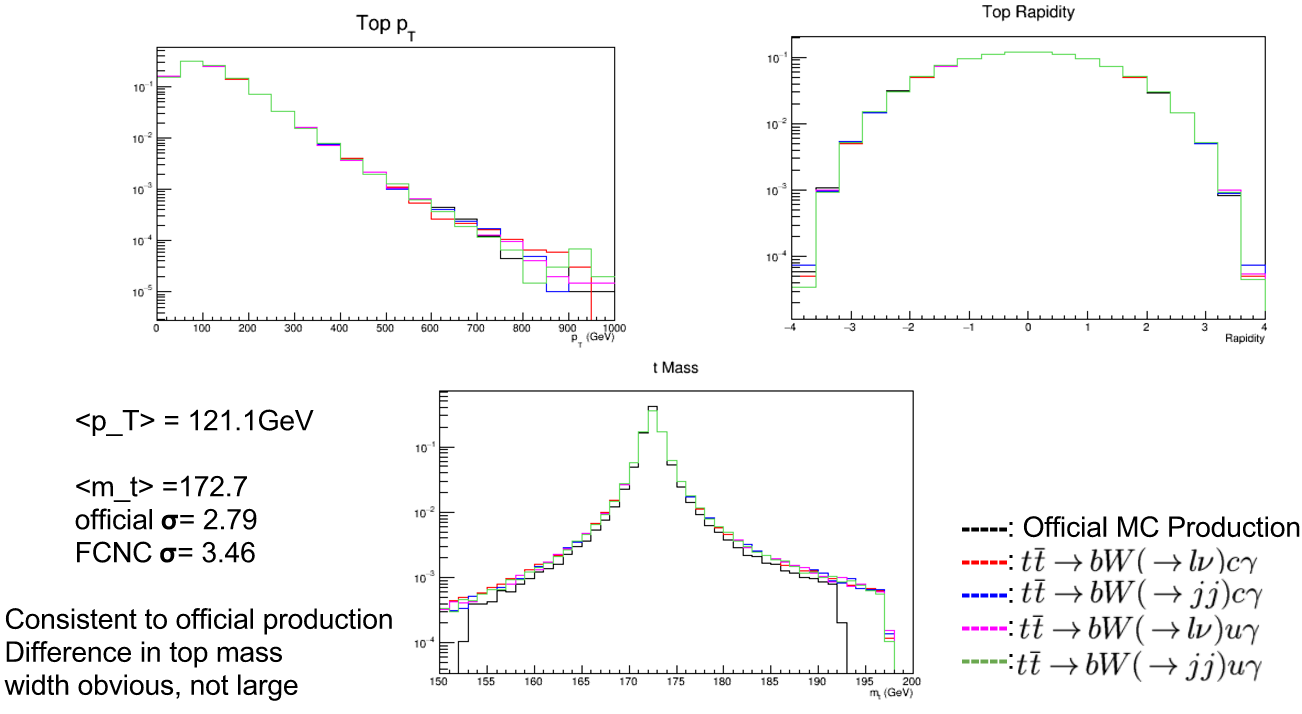
\includegraphics[width=1.\textwidth]{../../Thesis/ThesisImages/FCNCValidation.png}
}

\frame{\frametitle{MadGraph Issues May-October}
\begin{itemize}
\item Solved Issue in: \href{https://its.cern.ch/jira/browse/ATLMCPROD-6008}{[Production Request - ATLMCPROD-6008]}
\item Local (lxplus) version of MCProd19.2.5.33.4 had MadGraphControl-00-05-79, worked locally, not on grid
\item MadGraph version included in cache of MCProd19.2.5.34.1 with MadGraphControl-00-05-82 crashes locally, and on grid
\item Use of MCProd19.2.5.34.1 with correct MadGraph production runs locally and on grid
\item Pointed to MadGraphControl issue, something was rolled back or not changed when rolled out to grid sites, not seen until my production
\end{itemize}
\centering
\begin{columns}
\begin{column}{0.5\textwidth}
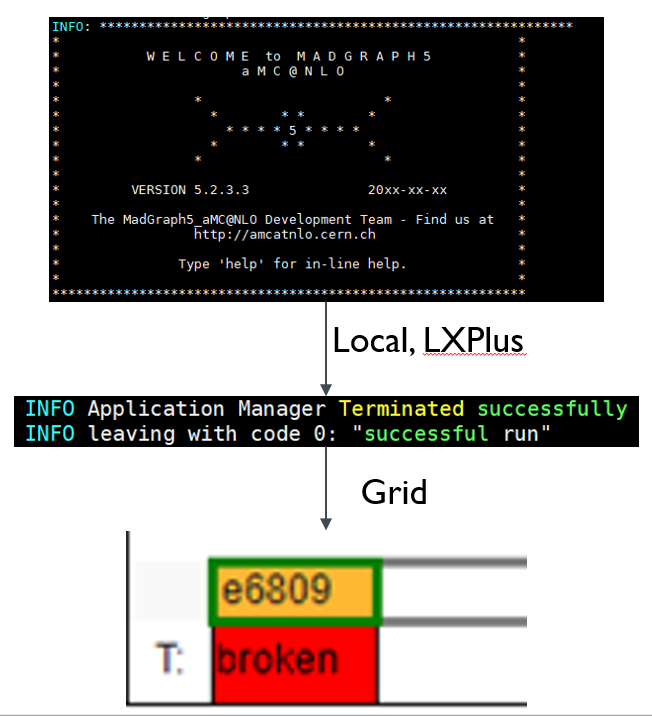
\includegraphics[width=.6\textwidth]{GridFail.png}
\end{column}
\begin{column}{0.5\textwidth}
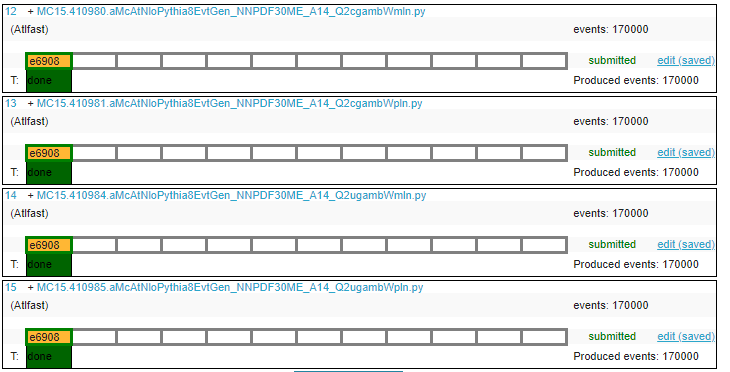
\includegraphics[width=1.\textwidth]{GridSuc.png}
\end{column}
\end{columns}
}

\subsection{Duplicate Event Removal}

\frame{\frametitle{Duplicate Event Removal}
\begin{itemize}
\item Due to the large influence of photons on this analysis special samples are used for major backgrounds
\begin{itemize}
\item $t\bar{t}+\gamma$ and V+jets+$\gamma$
\item Increases MC statistics for samples with prompt photons from the hard interation
\end{itemize}

\end{itemize}
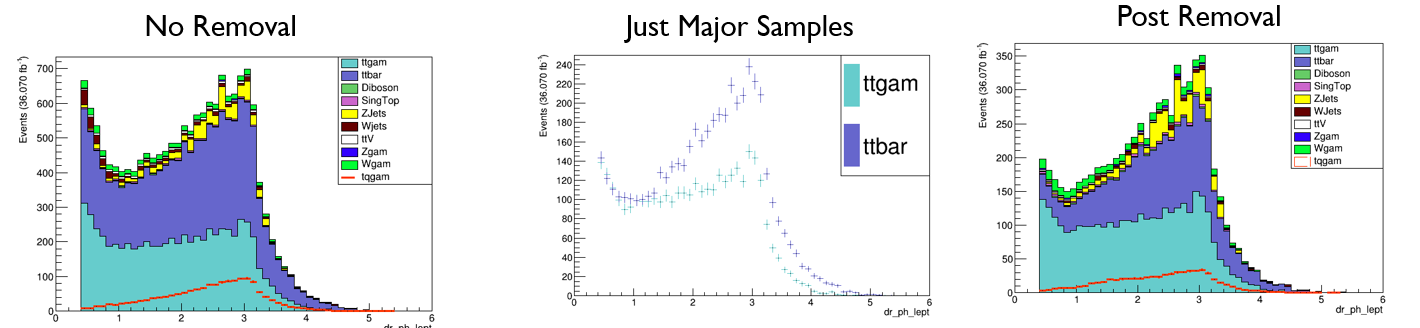
\includegraphics[width=1.\textwidth]{OldOVR.png}
\captionof{figure}{Schematic of how this worked with older samples, similar algorithm different implementation}
}
\frame{\frametitle{Duplicate Event Removal cont.}
\begin{itemize}

\item Release 21: Use MCTruthClassifier to determine origin of photons in event and directly determine if the photons are a result of an electron or jet faking a photon
\item The removal ensure events from  $t\bar{t}+\gamma$ and V+jets+$\gamma$ only contribute events from the hard scattering process and $t\bar{t}$, W+jets,Z+Jets only contribute events with a photon faked by an electron or a jet.
\item This hard scatter truth origin forces orthogonality and prevents duplicate events entering the selections
\item Currently nontrivial to update $N_{MC events}$ during event removal due to parallelization
\end{itemize}
\[w = \frac{\mathcal{L}. \sigma}{N_{MC events}}  \]

}

%%%%%%%%%%%%%%%%%%%%%%%%%%%%%%%%%%%%%%%%%%%%%%%%%%%%%%%%%%%%%%%%%
\section{Searching for Flavor Changing Neutral Current Signatures}

\subsection{FCNCs with Photons}

\subsection{Object Preselection Cuts}


\frame{\frametitle{Object Preselection}
\begin{itemize}
\item We preselect events with objects that look like similar to our expected topology
\item Require:
	\begin{itemize}
	\item Exactly one lepton (e or $\mu$) $\geq$ 28 GeV
	\item Exactly one Good photon $\geq$ 15GeV
	\item Missing Transverse Energy $\geq$ 30GeV
	\item $\geq 2$ Jets
	\end{itemize}
\item All following plots will have signal scaled to $1\%$ of inclusive $\sigma_{t\bar{t}}$, MC scaled to $36.21fb^{-1}$
\end{itemize}
}



\frame{\frametitle{Preselection Objects with $N_{BJet}\geq 1$ }
\begin{columns}
\begin{column}{0.02\textwidth}

\rotatebox{90}{Muon Channel \qquad  Electron Channel} 
%\rotatebox{90}{Muon Channel        } 
\end{column}
\begin{column}{0.33\textwidth}
\begin{itemize}
\item  Leading Jet $p_T$
\end{itemize}
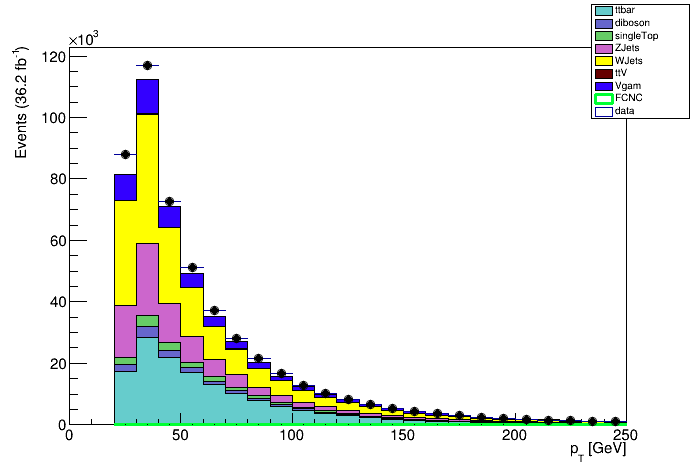
\includegraphics[width=1.1\textwidth]{{C:/Users/JTBar/Desktop/Research/FCNCAnalysis/plots/r21Plots/plotsMaybeOK/AllWeightsNonePreSelNoData/plots/el.presel.preselh_leadJet_pt}.png} \\
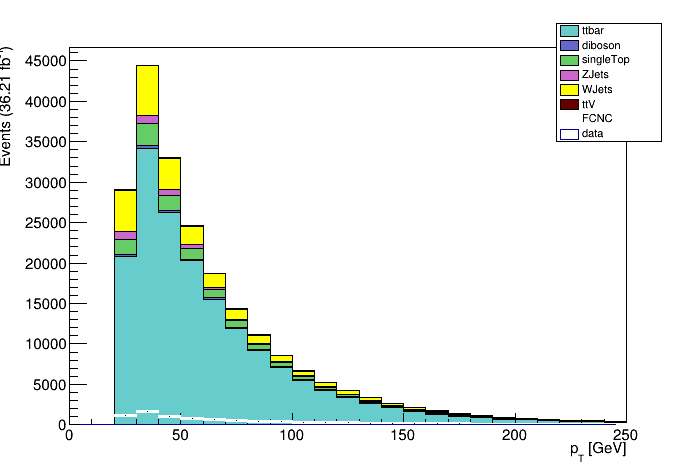
\includegraphics[width=1.1\textwidth]{{C:/Users/JTBar/Desktop/Research/FCNCAnalysis/plots/r21Plots/plotsMaybeOK/AllWeightsNonePreSelNoData/plots/mu.presel.preselh_leadJet_pt}.png}
\end{column}
\begin{column}{0.33\textwidth}
\begin{itemize}
\item Photons
\end{itemize}
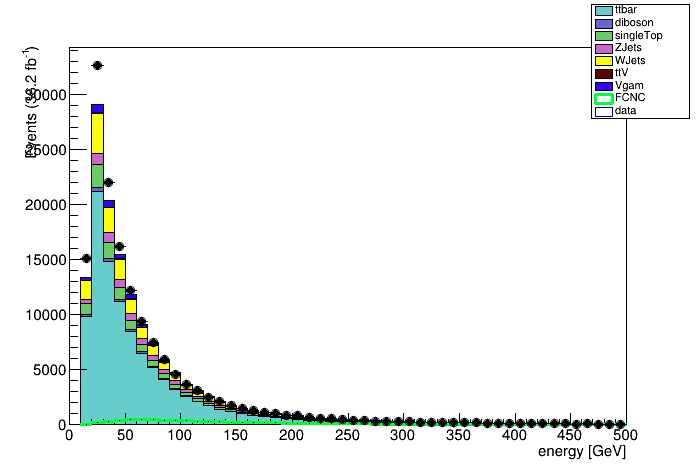
\includegraphics[width=1.1\textwidth]{{C:/Users/JTBar/Desktop/Research/FCNCAnalysis/plots/r21Plots/plotsMaybeOK/AllWeightsNonePreSelNoData/plots/el.presel.preselh_photon_e}.png} \\
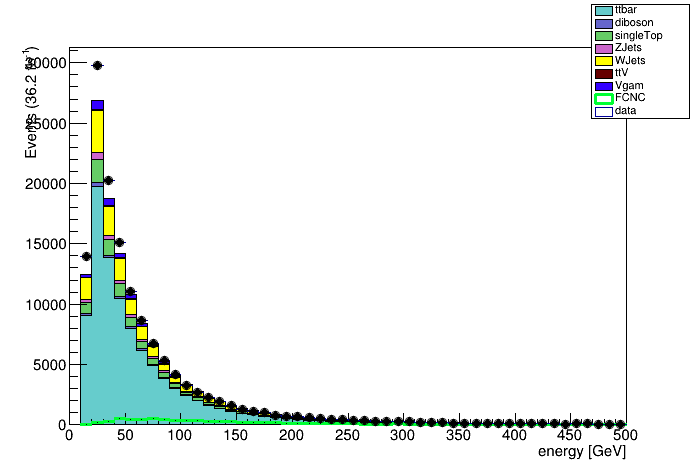
\includegraphics[width=1.1\textwidth]{{C:/Users/JTBar/Desktop/Research/FCNCAnalysis/plots/r21Plots/plotsMaybeOK/AllWeightsNonePreSelNoData/plots/mu.presel.preselh_photon_e}.png}
\end{column}
\begin{column}{0.33\textwidth}
\begin{itemize}
\item Leptons
\end{itemize}
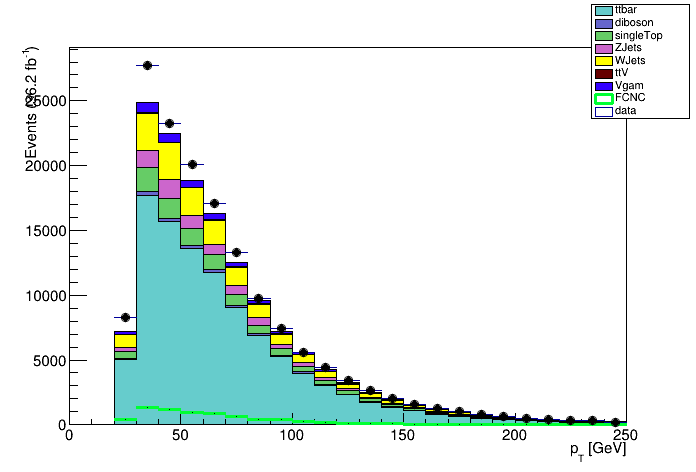
\includegraphics[width=1.1\textwidth]{{C:/Users/JTBar/Desktop/Research/FCNCAnalysis/plots/r21Plots/plotsMaybeOK/AllWeightsNonePreSelNoData/plots/el.presel.preselh_lepton_pt}.png} \\
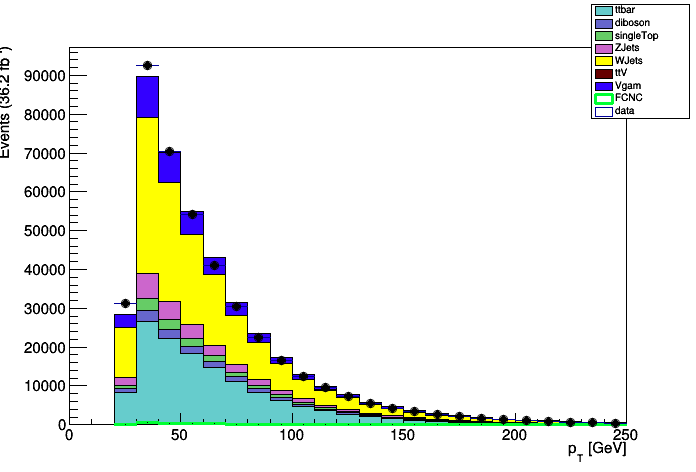
\includegraphics[width=1.1\textwidth]{{C:/Users/JTBar/Desktop/Research/FCNCAnalysis/plots/r21Plots/plotsMaybeOK/AllWeightsNonePreSelNoData/plots/mu.presel.preselh_lepton_pt}.png}
\end{column}
\end{columns}

 Bug with Normalization Factor that had been working for previous athena release, $t\bar{t}$ and $t\bar{t}+\gamma$ weights too large
}


\subsection{Top and Neutrino Reconstruction}
\frame{\frametitle{Where are the Tops?}
\begin{itemize}
\item Must be 'reconstructed' from these objects as well as b-jets and $E_T^{miss}$
\item $E_T^{miss}$ is calculated to balance the event energy in the transverse plane of the detector
\item The other particles are combined in the only way the signal topology would allow two top quark candidates
\begin{itemize}
\item Standard model top candidate: b-jet + lepton + neutrino 
\item FCNC Top: Photon + Light Jet
\end{itemize}
\end{itemize}
}

%%%%%%%%%%%%%%%%


\frame{\frametitle{Neutrinos}
\begin{itemize}
\item All missing energy in signal topology is from neutrino
\item We have $E_T^{miss}$ and its' direction   
\begin{itemize}
\item Can calulate  $E_{Tx}^{miss}$ and  $E_{Ty}^{miss}$ easily
\item Ambiguous direction along the z-axis
\end{itemize}
\item A minimization of this $\chi^2$ will allow us to determine the z momentum of the neutrino: $\chi^2 = \frac{(m_{b,l,\nu}-m_t)^2}{\sigma^2_{SMtop}}+\frac{(m_{l,\nu}-m_W)^2}{\sigma^2_W} $
\end{itemize}

%\[ \chi^2 = \frac{(m_{b,l,\nu}-m_t)^2}{\sigma^2_{SMtop}}+\frac{(m_{l,\nu}-m_W)^2}{\sigma^2_W}  \]
\begin{columns}
\begin{column}{0.5\textwidth}
\centering
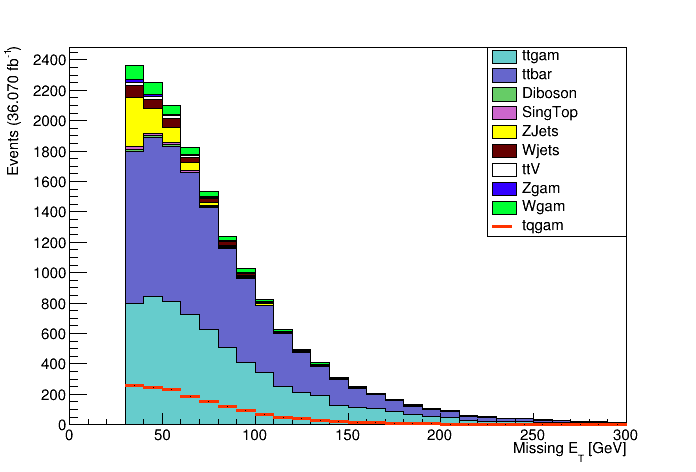
\includegraphics[width=.9\textwidth]{../../Thesis/ThesisImages/plotsloose/el_h_met_met.png}
\captionof{figure}{e-channel $E_T^{miss}$ distribution}
\end{column} 
\begin{column}{0.5\textwidth}
\centering
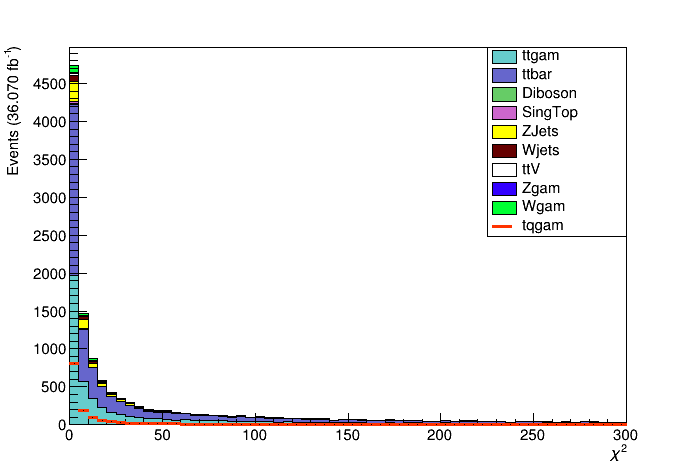
\includegraphics[width=.9\textwidth]{../../Thesis/ThesisImages/plotsloose/el_h_min_chi2.png}
\captionof{figure}{e-channel $\chi^2$ distribution}
\end{column}
\end{columns}
*Plots from previous release, same methodology used, same results
}
\subsection{Region Creation}
\frame{\frametitle{Validation Region - With Real Photons}
\begin{itemize}
\item Validation and Control Regions are created orthogonal to Signal Region for large backgrounds
\item VR for ($t\bar{t}+\gamma$)
\begin{itemize}
\item Same preselection and isolation cuts as SR
\item $>4$ jets
\item Reverse FCNC top mass cut $|m_{q\gamma}-m_{top}|>50GeV$: Gaurantees orthogonality 
\end{itemize}
\item VR for $W+\gamma$
\begin{itemize}
\item Similar preselection and isolation cuts to SR
\item = 0 BJets (orthogonal cut)
\end{itemize}
\item Similar regions have been created for regions without real photons - haven't included in grid runs yet for ease/size
\begin{itemize}
\item These regions include $t\bar{t}$ and $W$ rich samples with 0 good photons and different amounts of jets.
\end{itemize}
\end{itemize}
}

\frame{\frametitle{Example VR Plots - lepton $p_{T}$}
\begin{columns}
\begin{column}{0.02\textwidth}

\rotatebox{90}{Muon Channel \qquad  Electron Channel} 
%\rotatebox{90}{Muon Channel        } 
\end{column}
\begin{column}{0.48\textwidth}
\begin{itemize}
\item  VR1 - $W(V)+\gamma$ enriched
\end{itemize}
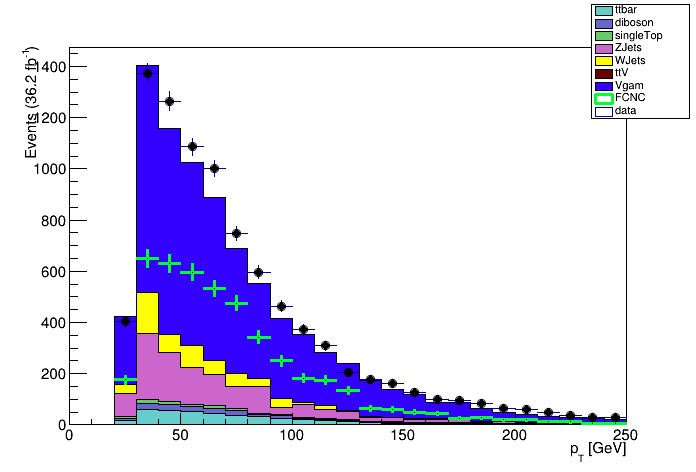
\includegraphics[width=.85\textwidth]{{C:/Users/JTBar/Desktop/Research/FCNCAnalysis/plots/r21Plots/plotsMaybeOK/AllWeightsAllReg/plots/el.VR1.VR1h_lepton_pt}.png} \\
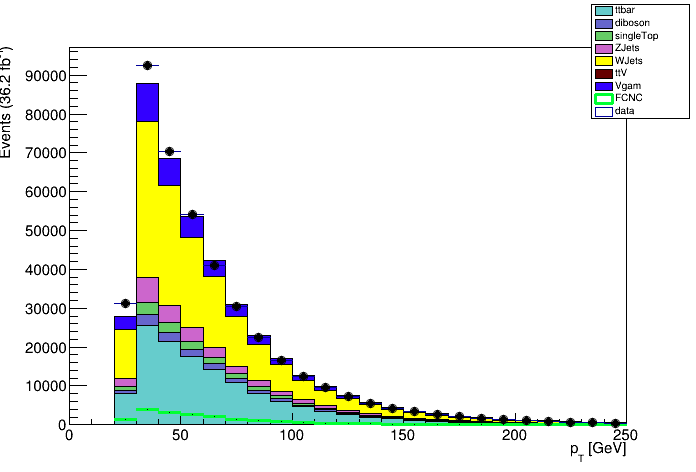
\includegraphics[width=.85\textwidth]{{C:/Users/JTBar/Desktop/Research/FCNCAnalysis/plots/r21Plots/plotsMaybeOK/AllWeightsAllReg/plots/mu.VR1.VR1h_lepton_pt}.png}
\end{column}
\begin{column}{0.48\textwidth}
\begin{itemize}
\item VR2 - $t\bar{t} + \gamma$ enriched
\end{itemize}
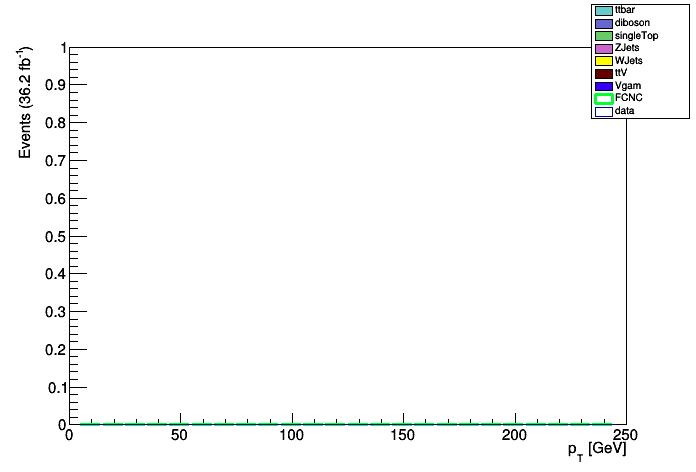
\includegraphics[width=.85\textwidth]{{C:/Users/JTBar/Desktop/Research/FCNCAnalysis/plots/r21Plots/plotsMaybeOK/AllWeightsAllReg/plots/el.VR2.VR2h_lepton_pt}.png} \\
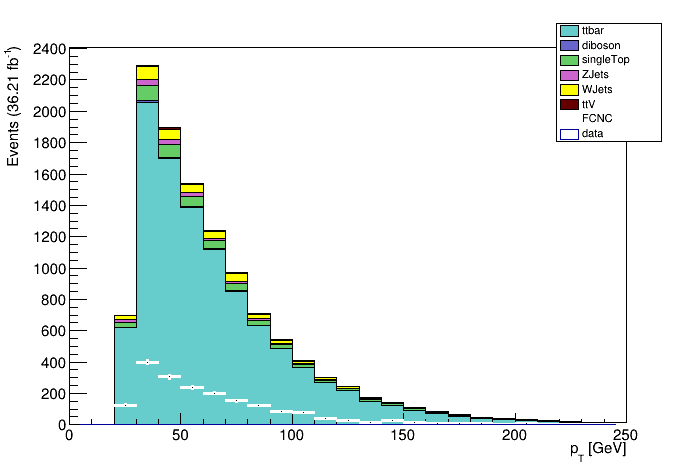
\includegraphics[width=.85\textwidth]{{C:/Users/JTBar/Desktop/Research/FCNCAnalysis/plots/r21Plots/plotsMaybeOK/AllWeightsAllReg/plots/mu.VR2.VR2h_lepton_pt}.png}
\end{column}

\end{columns}
}
\frame{\frametitle{Example VR Plots - n$_{Jets}$, n$_{BJets}$}
\begin{itemize}
\item Slightly more obvious to see problem with $t\bar{t} (+\gamma)$ samples 
\end{itemize}
\begin{columns}
\begin{column}{0.48\textwidth}
\begin{itemize}
\item  VR1 - $W(V)+\gamma$ enriched
\end{itemize}
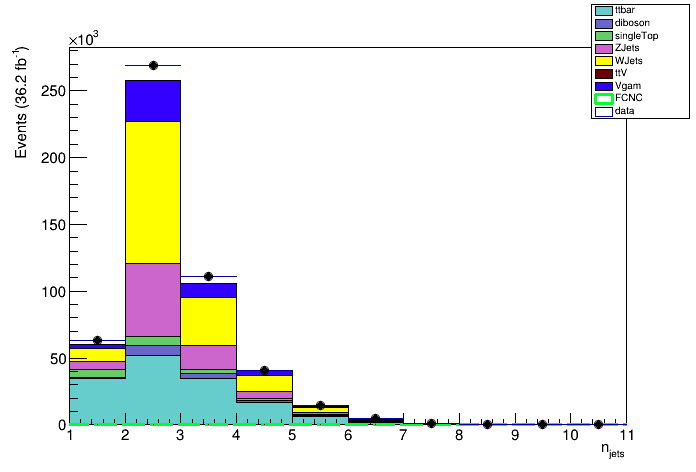
\includegraphics[width=.85\textwidth]{{C:/Users/JTBar/Desktop/Research/FCNCAnalysis/plots/r21Plots/plotsMaybeOK/AllWeightsAllReg/plots/el.VR1.VR1h_njets}.png}
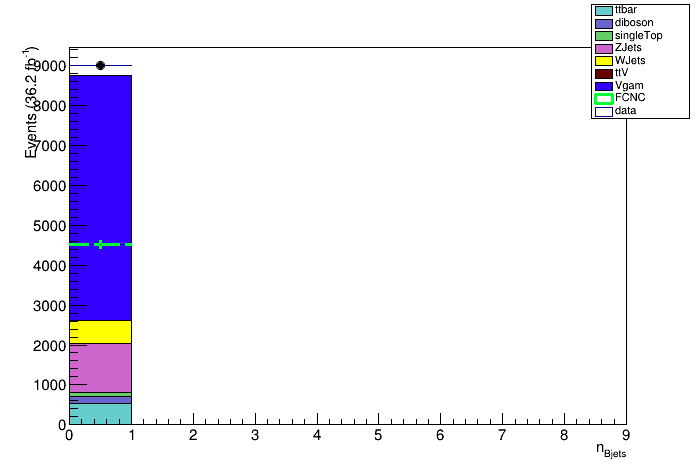
\includegraphics[width=.85\textwidth]{{C:/Users/JTBar/Desktop/Research/FCNCAnalysis/plots/r21Plots/plotsMaybeOK/AllWeightsAllReg/plots/el.VR1.VR1h_nBjets}.png}
\end{column}
\begin{column}{0.48\textwidth}
\begin{itemize}
\item VR2 - $t\bar{t} + \gamma$ enriched
\end{itemize}
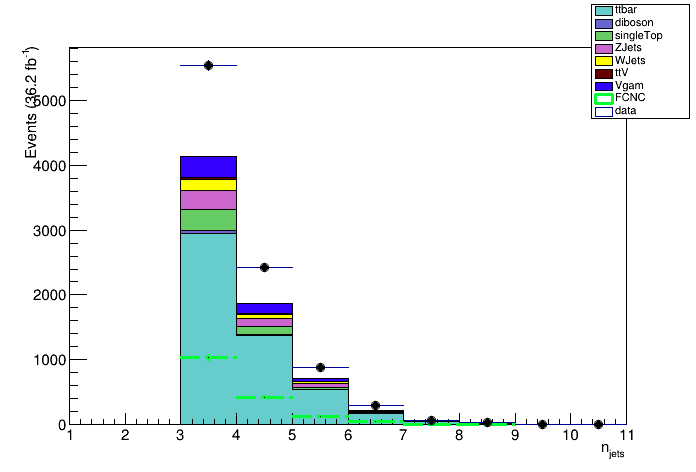
\includegraphics[width=.85\textwidth]{{C:/Users/JTBar/Desktop/Research/FCNCAnalysis/plots/r21Plots/plotsMaybeOK/AllWeightsAllReg/plots/el.VR2.VR2h_njets}.png} 
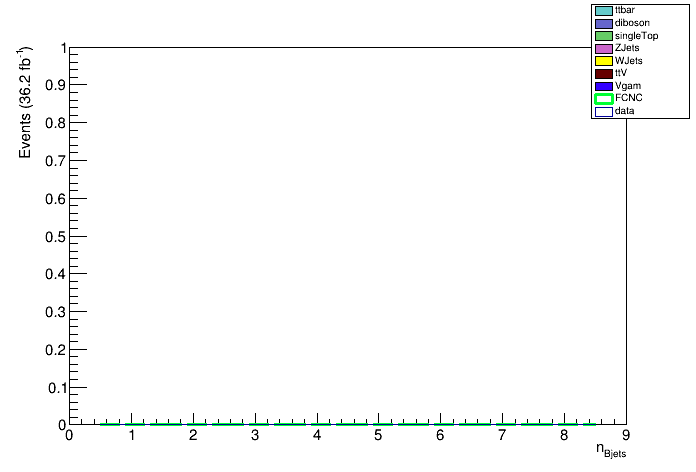
\includegraphics[width=.85\textwidth]{{C:/Users/JTBar/Desktop/Research/FCNCAnalysis/plots/r21Plots/plotsMaybeOK/AllWeightsAllReg/plots/el.VR2.VR2h_nBjets}.png}
\end{column}

\end{columns}
}
%\frame{\frametitle{VR Region expectations}
%\begin{itemize}
%\item Test
%\end{itemize}
%\begin{columns}{0.48\textwidth}
%\begin{itemize}
%\item VR1
%\end{itemize}
%\includegraphics[width=0.85\textwidth]{}
%\end{column}
%\begin{column}{0.48\textwidth}
%\begin{itemize}
%\item VR2
%\end{itemize}
%\includegraphics[width=0.85\textwidth]{}
%\end{column}
%\end{columns}
%
%}

%%%%%%%%%%%%%%%%%%%%%%%%%%%%%%%%%%%%%%%%%%%%%%%%%%%%%%%%%%%%%%%%%%
\section{Outlook and Conclusions}

\frame{\frametitle{Outlook}
\begin{itemize}
\item Still lots to be done
\begin{itemize}
\item Bug fixes on event normalizations
\item New duplicate event removal is most likely culprit at this point - nontrivial fix to implement
\item Further investigation into SR optimization with cuts on other variables such as $\Delta R_{\gamma, close jet}$ l
\end{itemize}
\item Fake Rates $e\rightarrow\gamma$ and $k\rightarrow\gamma$ will be investigated soon
\begin{itemize}
\item  MCTruthClassifier implemented already, should be straight forward
\end{itemize}
\item A new grid run will be done soon with MC16a and MC16d samples
\begin{itemize}
\item Inclusion of 0 photon events in grid sample for remaining control/validation regions
\end{itemize}
\item Full Analysis transitioned to be able to run on condor nodes
\begin{itemize}
\item  Capable of handling much larger samples by directly using grid output files
\item Necessary to look at MC16a/d/e samples and full 2018 data set in a reasonable amount of time
\end{itemize}
\end{itemize}
}



\frame{\frametitle{Conclusion}
\begin{itemize}
\item Any excess signal would be indicative of some physics beyond the Standard Model that couples strongly to the top sector
\item The search for FCNCs with enhanced rates are important pieces of testing many new theories
\item Hopefully no one else has to deal with a multimonth debugging process to get MC samples produced with MadGraph again
\item Now that I have my new samples the analysis can once again move forward
\item Thank you!
\end{itemize}
}


%%%%%%%%%%%%%%%%%%%%%%%%%%%%%%%%%%%%%%%%%%%%%%%%%%%%%%%%%%%%%%%%

\appendix
\section{Backup}
\frame{\frametitle{Backup}
}
\frame{\frametitle{Integrated Luminosity}
\centering
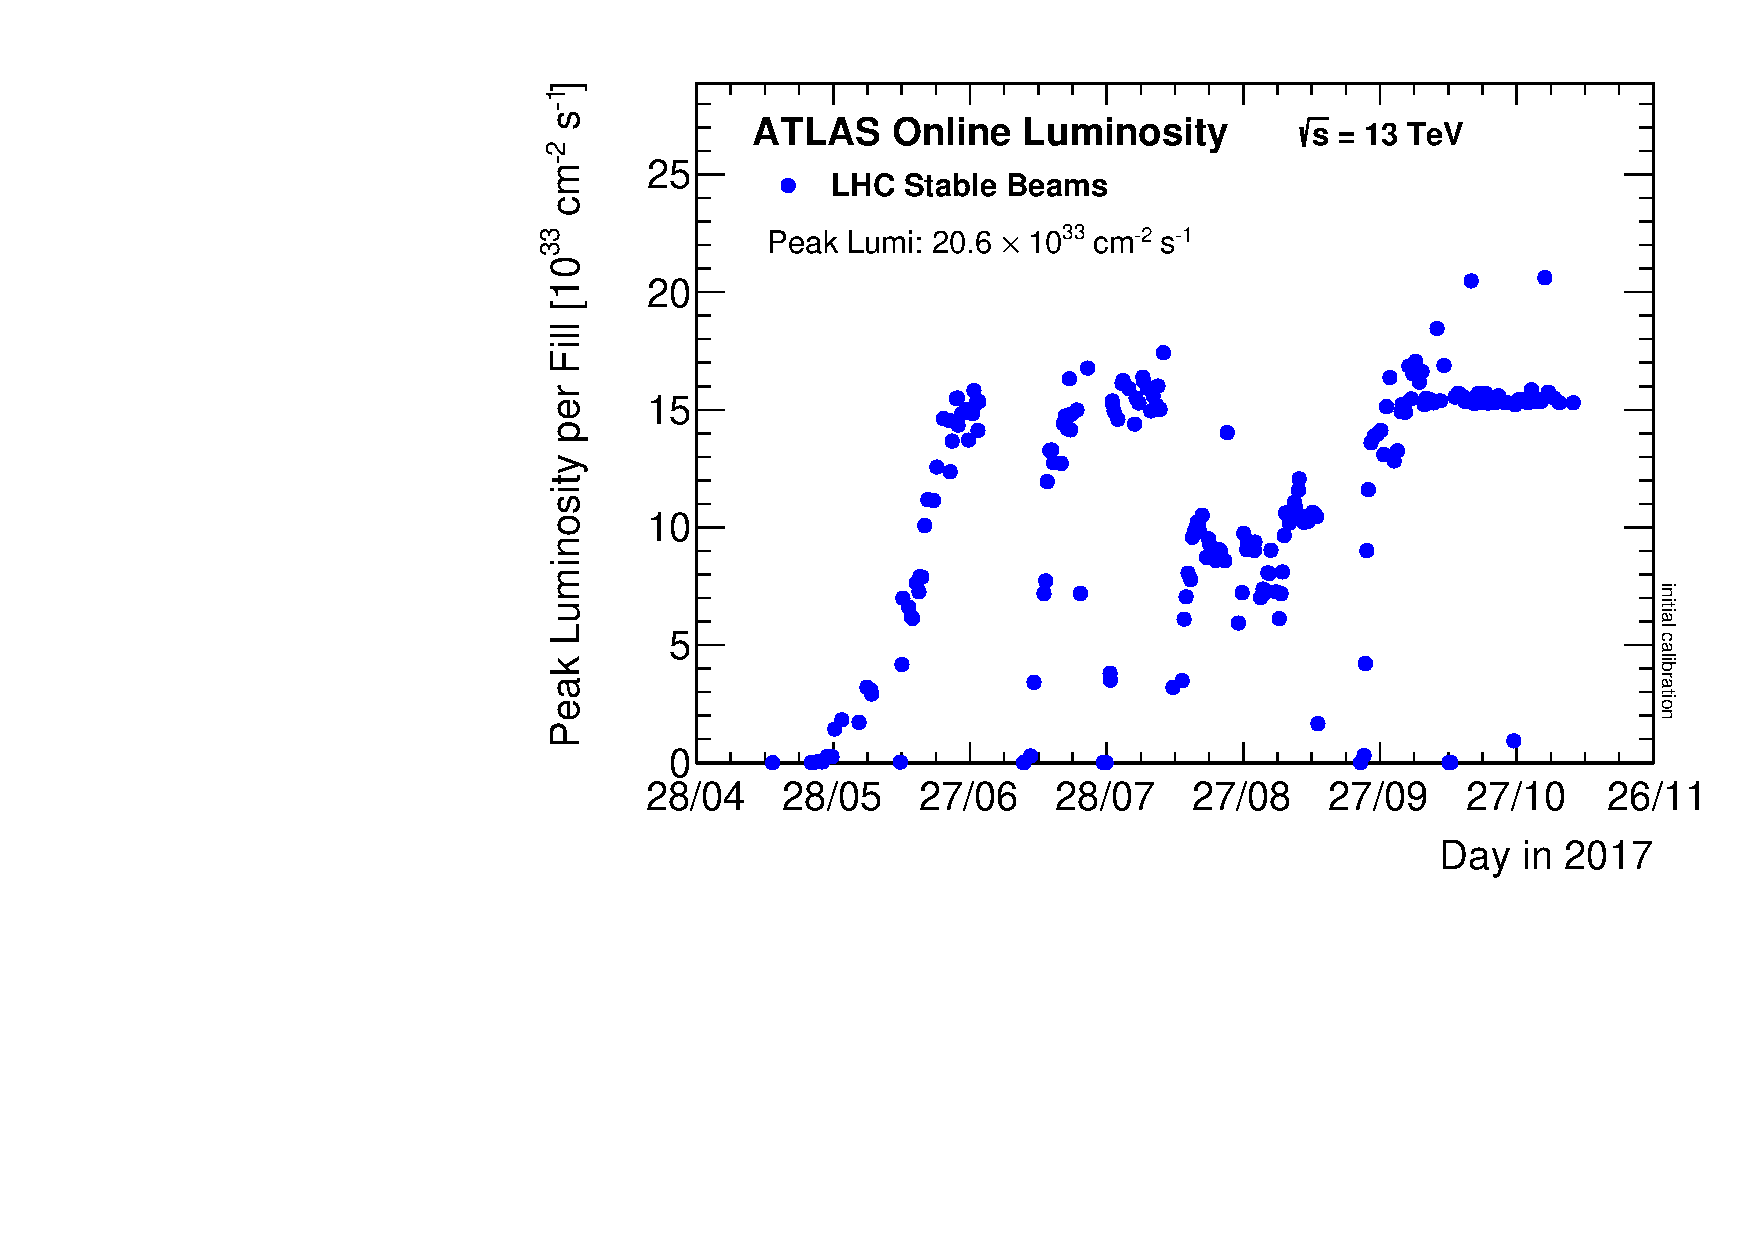
\includegraphics[width=1.\textwidth]{../../Thesis/ThesisImages/2017PeakLumiByFill.pdf}
}
\frame{\frametitle{A Couple BSM Diagrams}
\centering
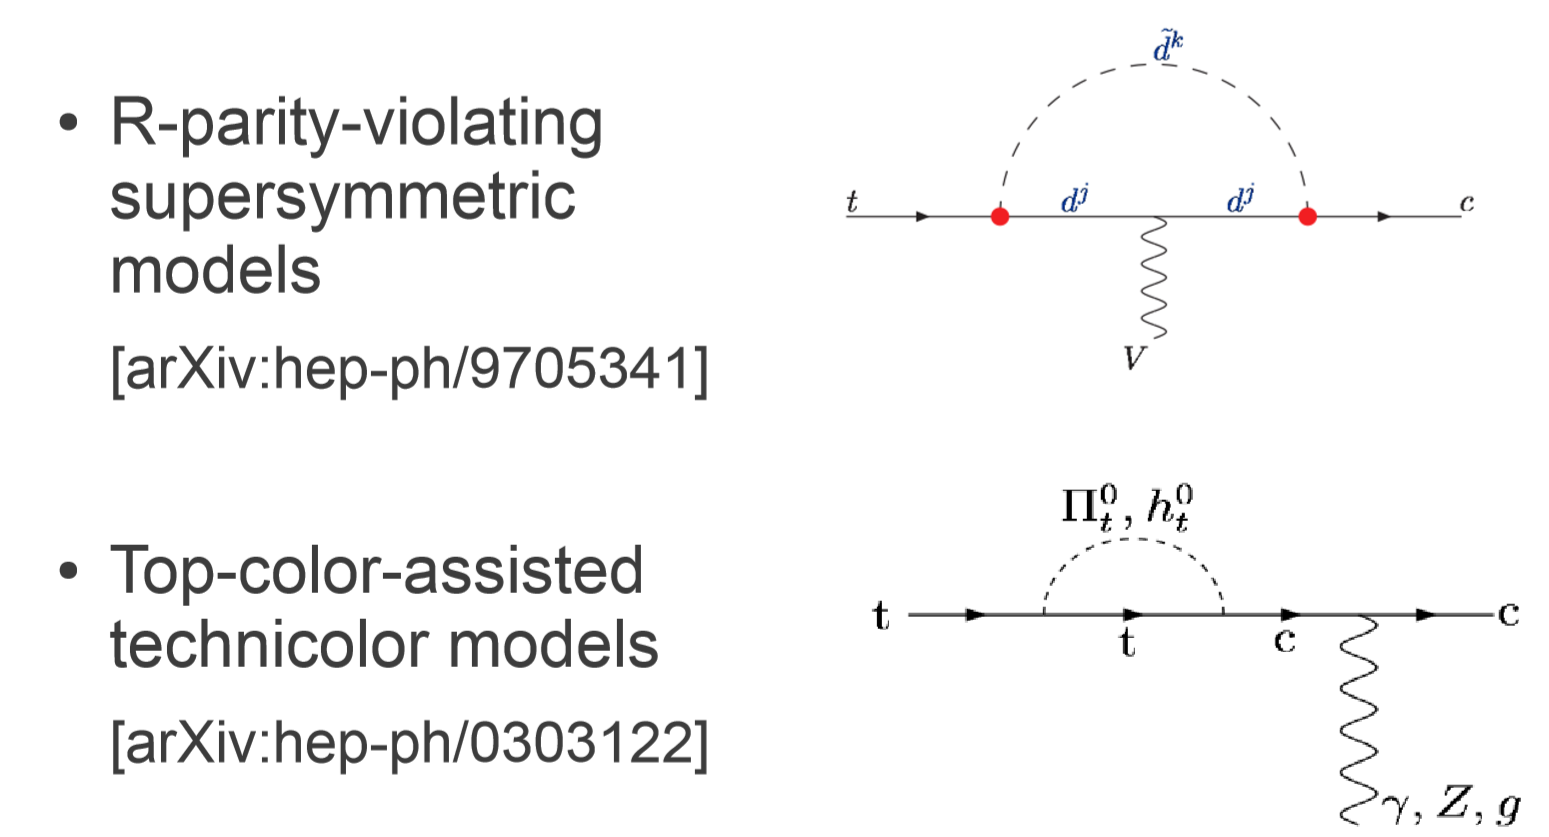
\includegraphics[width=1.\textwidth]{../../Thesis/ThesisImages/BSMDiagrams.png}
}

\frame{\frametitle{Jets/AntiKT}

\[ d_{ij} = min(\frac{1}{p_{ti}^2},\frac{1}{p_{tj}^2}) \frac{\Delta_{ij}^2}{R^2}
\]
\[ d_{iB} = \frac{1}{p_{ti}^2}
\]
\[ \Delta_{ij}^2 = (\eta_i -\eta_j )^2 + (\phi_i - \phi_j )^2
\]
\begin{itemize}
\item Find minimum of entire set of $\{ d_{ij},d_{iB} \}$
\item If $d_{ij}$ is the minimum particles i,j are combined into one particle and removed from the list of particles
\item If $d_{iB}$ is the minimum i is labelled as a final jet and removed from the list of particles
\item Repeat until all particles are part of a jet with distance between jet axes $\Delta_{ij}$ is greater than R
\end{itemize}
}

\frame{\frametitle{B-tagging}
\centering
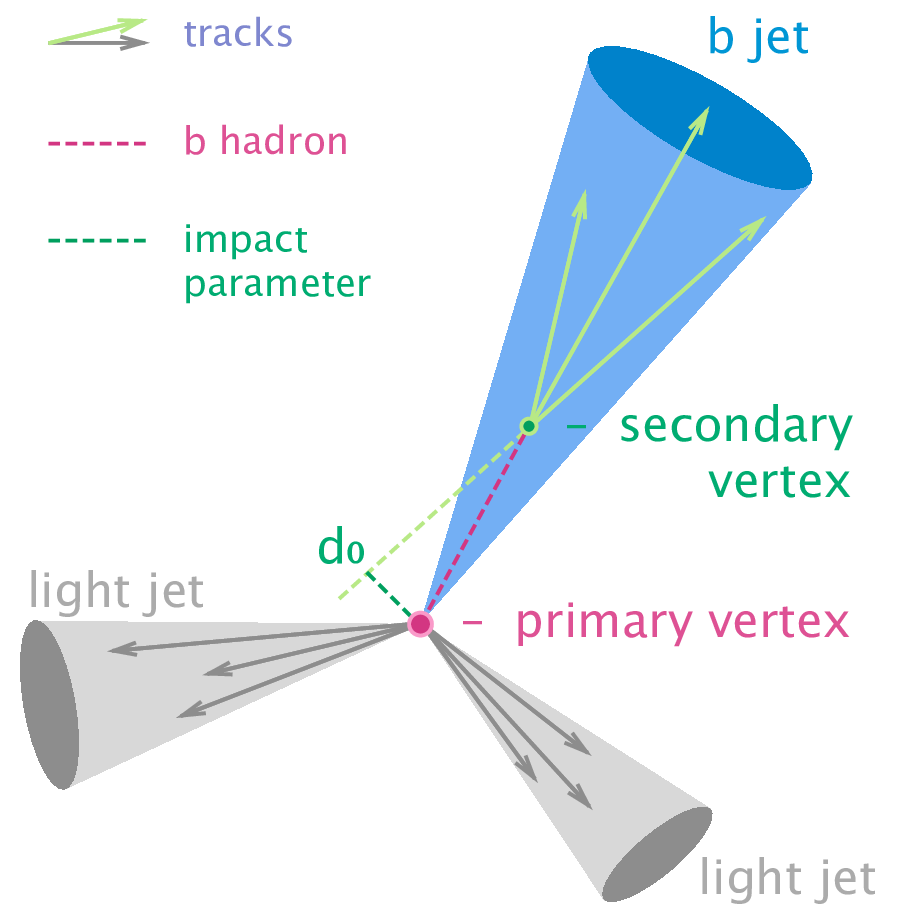
\includegraphics[height=.8\textheight]{../../Thesis/ThesisImages/B-tagging_diagram.png}

}
\frame{\frametitle{}
\[ \mathcal{L}^{eff}_{tq\gamma} = - e \bar{c} \frac{i \sigma^{\mu\nu}q_{\nu}}{m_t}(\lambda^{L}_{ct}P_L + \lambda^{R}_{ct}P_{R}) t A_{\mu} +H.c.
\]
}

\end{document}

%36.070
